\documentclass[10pt, letterpaper]{article}
\usepackage[includehead, margin=1in]{geometry}
\usepackage{fancyhdr}
\usepackage[british]{babel}
\usepackage{sansmathfonts}
\usepackage{stix}
\usepackage{soul}
\usepackage{color}
\usepackage{colortbl}
\usepackage{lewis}
\usepackage{siunitx}
\usepackage{textgreek}
\usepackage{mhchem}
\usepackage{modiagram}
\usepackage{tikzorbital}
\usepackage{chemfig}
\usepackage{hyperref}
\usepackage{xspace}
\usepackage{graphicx}
\graphicspath{{./assets/}}
\definecolor{error}{rgb}{255,255,0}
\newcommand{\degree}{\ensuremath{{}^{\circ}}\xspace}
\newcommand{\email}[1]{\href{mailto:#1}{\texttt{#1}}}

\begin{document}

\fancypagestyle{plain}{%
\fancyhf{}
\fancyhead[L]{CHEM 112--M01 \\ Dr.\@ Moulder}
\fancyhead[R]{H. Ryott Glayzer \\ 23 February 2024}
\fancyhead[C]{Assignment \\ \textit{Module 2.1}}
}


\title{Module 2.1 Homework}
\author{H. Ryott Glayzer}
\date{23 February 2024}


\maketitle

%%%%%%%%%%%%%%%%%%%%%%%%%%%%%%%%%%%%%%%%%%%%%%%%%%%%%%%%%%%%%%%%%%%%%%%%%%%%%%%
\section*{Notice of ADA Accommodation and Methods}
I have an ADA accommodation to do my assignment on paper.
This document is a utilization of that accommodation.
This assignment will utilize questions from the textbook,
\textit{Chemistry: Atoms First, 2e}, to practice the skills
and learning objectives for this class.
As a general statement, the textbook provides an answer key
to about half of the provided questions.
For ease of grading on behalf of Dr.\@ Moulder, 
I will do approximately every other
question with provided answers.
Any comments or concerns can be forwarded to my email at
\email{ryott.glayzer@mines.sdsmt.edu}.

\section*{Learning Objectives for Module 2.1}


Recognize the different types of chemical transformations: acid-base, precipitation, combination,
decomposition, single-replacement, oxidation-reduction, double replacement, and combustion.
(Chapter 4,5)


\begin{enumerate}
	\item Describe the basic properties of solutions (11.1)
	\item Distinguish electrolyte and nonelectrolyte solutions (chapter 11.1, 11.2)
	\item Identify common acids and bases (chapter 7.2)
	\item Derive chemical equations from narrative descriptions of chemical reactions.(chapter 7.1)
	\item Write and balance chemical equations in molecular, total ionic, and net ionic formats. (7.1)
	\item Define three common types of chemical reactions (precipitation, acid-base, and oxidation reduction) (chapter 7.2)
	\item Classify chemical reactions as one of these three types given appropriate descriptions or chemical equations (7.2)
	\item Predict the solubility of common inorganic compounds by using solubility rules. (chapter 7.2)
	\item Define oxidation, reduction, oxidizing agents, reducing agents, and oxidation numbers (chapter 7.2)
	\item Balance equations for oxidation-reduction reactions in acidic or basic solutions (chapter 7.2)
	\item Describe the reaction with oxygen of organic compounds, metals, and nonmetals (?)
	\item Explain the activity series of metals and use it to predict the product of a redox reaction involving a metal
\end{enumerate}


%%%%%%%%%%%%%%%%%%%%%%%%%%%%%%%%%%%%%%%%%%%%%%%%%%%%%%%%%%%%%%%%%%%%%%%%%%%%%%%
\section*{11.1: The Dissolution Process}

\subsection*{Q.1: How do solutions differ from compounds? From other mixtures?}
Compounds follow the law of Definite Proportions and will always be comprised
of a specific ratio of elements, while solutions can differ wildly in their
concentration.
A solution is a subset of mixtures that is necessarily homogeneous.

%%%%%%%%%%%%%%%%%%%%%%%%%%%%%%%%%%%%%%%%%%%%%%%%%%%%%%%%%%%%%%%%%%%%%%%%%%%%%%%

\subsection*{Q.5: Indicate the most important types of 
intermolecular attractions in each of the following reactions.}

\subsubsection*{5.a. The solution in Figure 11.2:}
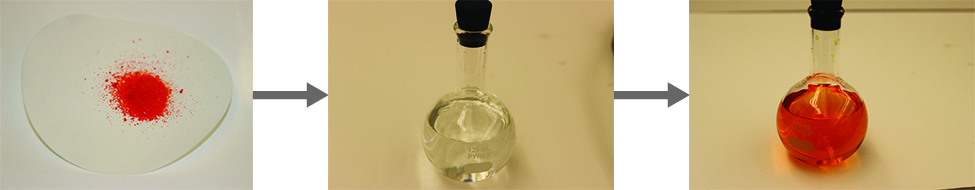
\includegraphics[width=\textwidth]{figure_11_2}
\begin{center}
	\large
	\textbf{%
		\ce{K2Cr2O7 (s) -> 2K^{+} (aq) + Cr2O7^{2-} (aq)}
	}
\end{center}
Ion-Dipole attraction

\subsubsection*{5.b.\@ \ce{NO (l)} in \ce{CO (l)}}
\textit{Isn't this only possible below like 75K?}
\\
Dipole-Dipole Attraction

\subsubsection*{5.c.\@ \ce{Cl2 (g)} in \ce{Br2 (l)}}
Dispersion

\subsubsection*{5.d.\@ \ce{HCl (g)} in benzene \ce{C6H6 (l)}}
Dispersion
\subsubsection*{5.e.\@ \ce{CH3OH (l)} in \ce{H2O (l)}}
\hl{I'm not sure.}

%%%%%%%%%%%%%%%%%%%%%%%%%%%%%%%%%%%%%%%%%%%%%%%%%%%%%%%%%%%%%%%%%%%%%%%%%%%%%%%
\section*{11.2: Electrolytes}
\subsection*{Q.9: Explain why the ions \ce{Na+} and \ce{Cl-} are strongly
solvated in water but not in hexane, a solvent composed of nonpolar molecules}
Sodium Chloride is a highly polar molecule and thus dissolves readily in polar
solvents, like water. This occurs because of the polar electronegativity
attractions between constituent ions. The nonpolar solvent does not act on 
the polarity of the sodium chloride and thus does not readily dissolve it.

\subsection*{Q.13: What is the expected electrical conductivity of the
following solutions?}
\begin{center}
	\begin{tabular}{|c|c|c|c|}
		\hline
		\ce{NaOH (aq)} & \ce{HCl (aq)} & \ce{C6H12O6 (aq)} & \ce{NH3 (aq)} \\
		\hline
		high & high & zero & low \\
		\hline
	\end{tabular}
\end{center}


%%%%%%%%%%%%%%%%%%%%%%%%%%%%%%%%%%%%%%%%%%%%%%%%%%%%%%%%%%%%%%%%%%%%%%%%%%%%%%%
\section*{7.1: Writing and Balancing Chemical Reactions}
\subsection*{Q.1: What does it mean to say on equation is balanced?
Why is it important for an equation to be balanced?}
An equation is balanced when the number of reactants and products for each
element is equal. It is important because the reaction would not otherwise 
adhere to the law of conservation of energy and matter.

\subsection*{Q.5: Write a balanced molecular equation describing each of the 
following chemical reactions.}
\subsubsection*{a: Solid calcium carbonate is heated and decomposes
to solid calcium oxide and carbon dioxide gas.}
\ce{CaCO3 (s) -> CaO (s) + CO2 (g)}
\subsubsection*{b: Gaseous butane, C4H10, reacts with diatomic oxygen gas
to yield gaseous carbon dioxide and water vapor.}
\ce{2C4H10 (g) + 13O2 (g) -> 8CO2 (g) + 10H2O (g)}
\subsubsection*{c. Aqueous solutions of magnesium chloride and sodium hydroxide
react to produce solid magnesium hydroxide and aqueous sodium chloride.}
\ce{MgCl2 (aq) + 2NaOH (aq) -> Mg (OH)2 (s) + 2NaCl (aq)}
\subsubsection*{d. Water vapor reacts with sodium metal to produce
solid sodium hydroxide and hydrogen gas.}
\ce{2H2O (g) + 2 Na (s) -> 2NaOH (s) + H2 (g)}

\subsection*{Q.9: Aqueous hydrogen fluoride (hydrofluoric acid) is used to
etch glass and to analyze minerals for their silicon content.
Hydrogen fluoride will also react with sand (silicon dioxide).}
\subsubsection*{a: Write an equation for the reaction of solid silicon dioxide
with hydrofluoric acid to yield gaseous silicon tetrafluoride and liquid water.}
\ce{4HF (aq) + SiO2 (s) -> SiF4 (g) + 2H2O (l)}
\subsubsection*{b: The mineral fluorite (calcium fluoride) occurs extensively
in Illinois. Solid calcium fluoride can also be prepared by the reaction of
aqueous solutions of calcium chloride and sodium fluoride, yielding
aqueous sodium chloride as the other product.
Write complete and net ionic equations for this reaction.}
\ce{2Na+ (aq) + 2F- (aq) + Ca^{2+} (aq) + 2Cl- (aq) -> CaF2 (s) + 2Na+ (aq) + 2Cl- (aq)}
\\\ce{2F- (aq) + Ca^{2+} -> CaF2 (s)}
%%%%%%%%%%%%%%%%%%%%%%%%%%%%%%%%%%%%%%%%%%%%%%%%%%%%%%%%%%%%%%%%%%%%%%%%%%%%%%%
\section*{7.2: Classifying Chemical Reactions}
\subsection*{Q.13: Indicate what type, or types,
of reaction each of the following represents:}
\subsubsection*{\ce{Ca (s) + Br2 (l) -> CaBr2 (s)}}
Redox addition
\subsubsection*{\ce{Ca (OH)2 (aq) + 2HBr (aq) -> CaBr2 (aq) + 2H2O (l)}}
Acid-Base Neutralization 
\subsubsection*{\ce{C6H12 (l) + 9O2 (g) -> 6CO2 (g) + 6H2O (l)}}
Redox Combustion
\subsection*{Q.17: Determine the oxidation states of the elements in the
compounds listed. None of the oxygen-containing
compounds are peroxides or superoxides.}
\subsubsection*{\ce{H3PO4}}
\begin{center}
	\begin{tabular}{|c|c|c|}
		\hline
		H & P & O \\
		\hline
		+1 & +5 & -2 \\
		\hline
	\end{tabular}
\end{center}
\subsubsection*{\ce{Al (OH)3}}
\begin{center}
	\begin{tabular}{|c|c|c|}
		\hline
		Al & H & O \\
		\hline
		+3 & +1 & -2 \\
		\hline
	\end{tabular}
\end{center}
\subsubsection*{\ce{SeO2}}
\begin{center}
	\begin{tabular}{|c|c|}
		\hline
		Se & O \\
		\hline
		+4 & -2 \\
		\hline
	\end{tabular}
\end{center}
\subsubsection*{\ce{KNO2}}
\begin{center}
	\begin{tabular}{|c|c|c|}
		\hline
		K & N & O \\
		\hline
		+1 & +3 & -2 \\
		\hline
	\end{tabular}
\end{center}
\subsubsection*{\ce{In2S3}}
\begin{center}
	\begin{tabular}{|c|c|}
		\hline
		In & S \\
		\hline
		+3 & -2 \\
		\hline
	\end{tabular}
\end{center}
\subsubsection*{\ce{P4O6}}
\begin{center}
	\begin{tabular}{|c|c|}
		\hline
		P & O \\
		\hline
		+3 & -2 \\
		\hline
	\end{tabular}
\end{center}
\subsection*{Q.21: Complete and balance the following acid-base equations:}
\subsubsection*{\ce{HCl (g) + Ca (OH)2 (s)}}
\ce{2HCl (g) + Ca (OH)2 (s) -> CaCl2 (s) + 2H2O (l)}
\subsubsection*{\ce{Sr (OH)2 (aq) + HNO3 (aq)}}
\ce{Sr (OH)2 (aq) + 2HNO3 (aq) -> Sr (NO3)2 (aq) + 2H2O (l)}
\subsection*{Q.25: Complete and balance the equations for the following
acid-base neutralization reactions. If water is used as a solvent,
write the reactants and products as aqueous ions.
In some cases, there may be more than one correct answer,
depending on the amounts of reactants used.}
\subsubsection*{\ce{Mg (OH)2 (s) + HClO4 (aq) ->}}
\ce{Mg (OH)2 (s) + 2HclO4 (aq) -> Mg^{2+} (aq) + 2ClO4- (aq) + 2H2O (l)}
\subsubsection*{\ce{SO3 (g) + H2O (l) ->}}
\ce{SO3 (g) + 2H2O (l) -> H3O^{+} (aq) + HSO4- (aq) + nH2SO4 (aq)}
\subsubsection*{\ce{SrO (s) + H2SO4 (l) ->}}
\ce{SrO (s) + H2SO4 (l) -> SrSO4 (s) + H2O}
\subsection*{Q.29: Great Lakes Chemical Company produces bromine, Br2, from
bromide salts such as NaBr, in Arkansas brine by treating the brine with
chlorine gas. Write a balanced equation for the reaction of NaBr with Cl2.}
\ce{2NaBr (aq) + Cl2 (g) -> 2NaCl (aq) + Br2 (l)}
\subsection*{Q.33: Complete and balance the equations of the following
reactions, each of which could be used to remove hydrogen sulfide
from natural gas:}
\subsubsection*{\ce{Ca (OH)2 (s) + H2S (g) ->}}
\ce{Ca (OH)2 (s) + H2S (g) -> CaS 9S0 + 2H2O (l)}
\subsubsection*{\ce{Na2CO3 (aq) + H2S (g) ->}}
\ce{Na2CO3 (aq) + H2S (g) -> Na2S (aq) + CO2 (g) + H2O (l)}


\section*{Grading}

$\frac{35}{36}$ points earned, or $97\%$
















\end{document}





%%%%%%%%%%%%%%%%%%%%%%%%%%%%%%%%%%%%%%%%%%%%%%%%%%%%%%%%%%%%%%%%%%%%%%%%%%%%%%%
%%%                                 Copypasta                               %%%
%%%%%%%%%%%%%%%%%%%%%%%%%%%%%%%%%%%%%%%%%%%%%%%%%%%%%%%%%%%%%%%%%%%%%%%%%%%%%%%

% Table for questions with multiple parts

% \begin{center}
% 	\begin{tabular}{|c|c|c|c|c|}
% 		\hline
% 		_ & _ & _ & _ & _ \\
% 		\hline
% 		_ & _ & _ & _ & _ \\
% 		\hline
% 	\end{tabular}
% \end{center}
